%Describe the overall structure of the system, the different components of the system and interfaces between these.
\chapter{Overall Design} %Carsten
Here we describe each component needed in the implementation. We detail the requirements and uses of each component, as well as argue for their existence. This chapter was informally described during development, used in the implementation, but also serves as a rough description of the overall system.

\section{Objects} %Carsten
Everything in the game-space is a \emph{prop}. These are the objects which the physics engine manipulates. Each of them contains a \emph{hitbox}, a rectangular square used to calculate collisions. They also contain graphical information needed to be drawn.
\newline
Next we have \emph{units}, which consists of all enemies and the player. All units are props, and are part of the physics engine. The difference is that a unit also has an AI to update. As a side note, we did not name them "actors" in suit of the theatrical names, scenes and props, since it would be confusing that all actors are props.
\newline
The only reason we created units on top of props is because of \emph{coins}. These grant the player a score bonus when collected. The reason for coins to extend props is to reuse collision code, and makes them affected by the physics engine as a bonus.
\newline
Two kinds of unit extensions exist: the \emph{minotaur} and the \emph{hero}. The former is the only implemented enemy type in the game and the latter is the unit controlled by the player. These contain graphical and gameplay data as well as their AI code. In case of the hero, his 'AI' is reading player input.

\subsection*{Minotaur AI} %Carsten
The AI needs to receive world information and deliver actions. This prompts a cyclic model-controller relationship, which aims to place as much freedom in the hands of the AI as possible. The biggest limiting factor is how complex the world is, most of all the physics engine. The AI cannot and should not predict how its actions would affect the world - this is the job of the physics engine. This limits us in how advanced the AI can be, especially when planning forward, since we cannot guarantee an action leads to the desired outcome. For example, if a unit would jump across a gap or on top of a platform, he would need to steer himself for several frames to land safely and surely. Moreover, planning further than the current frame would require the unit to have a concept of his jumping abilities, size, and world geometry.
\newline
This complexity leads us to create much simpler AI, one which does not plan ahead. A possible solution which was considered, would be preprocessing the map and generate paths through the map. This would be expensive in memory and code-size and would make implementing different enemy types problematic. We would be forced to either use similarly moving enemies or generate additional pathing maps for each enemy type. This would be a lot of work for only a bit smarter AI, and it was not a very enticing feature with such limited hardware.
\newline
The AI we settled with would simply move towards a given goal, jump if necessary, or wander aimlessly like enemies usually do in platforming games.
\newline
Communication between the unit and the scene is done by an object called \emph{logic}. This should contain all necessary methods and information needed by all unit types. A few examples would be the hero's position, whether or not a given prop is in the air, or whether a given space is 'walkable'. It would also need to execute actions given by the units, which are processed in the physics engine. So it handles collision detection, gravity and calls relevant methods in case a prop collides with a wall or is attacked.
\newline
As mentioned there is a cycle of dependencies: Logic requires scenes for map information, which includes units that need logic to communicate. We attempted to avoid cycles which could be a problem during implementation, but it seemed unavoidable when an informed AI is in play.

\subsection*{Hero Input} %Cebrail
The hero is a Greek warrior. Therefore he's capable of doing basic things like walking and running. To interact with enemies and navigate through the map he will need to duck, jump and attack. All these actions require that we have a proper input system.
\newline
To achieve this, we chose to use the Wii Nunchuk. It has one thumbstick and two buttons as well as a built-in accelerometer. We utilized the thumbstick to control the hero's horizontal movement and ducking maneuvers. The two buttons are used to jump and attack. To finish a map, the player attacks while ducking.
\newline
These button assignments were configured to what felt most comfortable.

\begin{figure}[H]
  \centering
  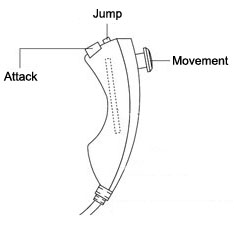
\includegraphics[scale=0.6]{Figures/nunchuk}
  \caption{Button assignments}
  \label{fig:Nunchuk}
\end{figure}

Here is an overview of how to control the hero.

\begin{table}[H]
    \centering
    \begin{tabular}{ll}
    Action               & Combination                \\ \hline
    Horizontal movement  & Thumbstick left and right  \\
    Jump                 & C Button                   \\
    Attack               & Z Button                   \\
    Duck                 & Thumbstick down            \\
    Exit map             & Thumbstick down + Z Button \\
    \end{tabular}
\end{table}


\section{Levels} %Carsten
The levels in the game are called \emph{scenes}. They contain the world geometry and all the props. The world is made out of square blocks called \emph{tiles}. There are multiple types of tiles, used to diversify the world and mark special locations. There are solid blocks, partially solid platforms, an entrance and an exit. The scene is composed of a \emph{grid} of tiles which contains exactly one entrance and exit. Each level is a climb to the top, with the entrance at the bottom and exit at the top. Minotaurs and coins are randomly placed around the map, though not too close to the entrance.
\newline
Initially, ladders were also supposed to be in the game, but their function would have overlapped with platforms. Ladders would be difficult to implement and would require specific animations for both the player and the enemies. They were cut from the game in favor of the easier to implement platforms.

\subsection*{Level Generation} %Carsten
The point of randomly generated maps is two fold: it vastly increases the replay-ability of a game, and it encourages more skilled play by forcing players to be better at the gameplay elements, rather than the specific levels included. We can ensure this if the maps are adequately different from each other, and if the range of possible maps is large enough. %Requirements?
\newline
More specifically, the level generation should return a new scene with a matching entrance and exit. The level should always be solvable, that is, there must be a path between the entrance and exit which the player can follow. It should not be possible to get stuck in the map, though it may contain unreachable places. Enemies and coins should be spread evenly around the map, though not too close to the entrance, where the hero would spawn. In addition to this, the level generation should be able to vary the difficulty, at least by varying the amount of enemies, to allow increasing the difficulty as the game progresses. %Requirements?
\newline
New maps are rarely needed compared to other code parts, so speed is not a priority. Memory and code size are the greater evils in this scenario.

\section{Graphics}%Philip
All the images used are either hand drawn from scratch or based off open source images which we altered. Each type of unit has a set of animations in the form of multiple images. These animations cycle through their sequences with respect to time. It is also set to every animation how many milliseconds should pass before moving on to the next image. There are conditions however that alter the standard procedure of sprite animating. One condition makes sure that an animation runs through to the end of the sequence before being able to change to a different animation. The other assures that it just stops at the end of the sequence and thereafter can't change to any other animation. The images are able to mirror horizontally for when props are facing different directions. They are positioned in such a way that their centers are at the same point as that of their respective hitbox. 


\subsection*{Sound} %Cebrail/Jonathan
We implemented sound effects on essential events. We agreed that it was what the game needed to provide a more immersive feel.\\
We wanted the sounds to come primarily from the hero's actions and interactions. We added sounds for jumping, attacking, exiting a map and collecting coins.\\
We would have included background music, but as mentioned previously, flash memory space was an issue and loading a music file uses too much.
